%%%%%%%%%%%%%%%%%%%%%%%%%%%%%%%%%%%%%%%%%%%%%%
%Lab report writeup based on template by Derek Hildreth
%%%%%%%%%%%%%%%%%%%%%%%%%%%%%%%%%%%%%%%%%%%%%%

%\documentclass[aps,letterpape,10pt]{revtex4}
\documentclass[aps,letterpaper,10pt]{article}
%\documentclass{article}

\usepackage{graphicx} % For images
\usepackage{float}    % For tables and other floats
\usepackage{verbatim} % For comments and other
\usepackage{amsmath}  % For math
\usepackage{amssymb}  % For more math
\usepackage{fullpage} % Set margins and place page numbers at bottom center
\usepackage{subfig}   % For subfigures
\usepackage[usenames,dvipsnames]{color} % For colors and names
\usepackage{fancyhdr} %headers
\usepackage{listings} %for code
\usepackage{color} %to color code
\usepackage{wrapfig} % for inline images

%Color and code setup
\definecolor{dkgreen}{rgb}{0,0.6,0}
\definecolor{gray}{rgb}{0.5,0.5,0.5}
\definecolor{mauve}{rgb}{0.58,0,0.82}
\definecolor{codebg}{rgb}{.95,.95,.98}

\lstset{ %
	language=Java,
	tabsize=4, 
	numbers=left,
	numberstyle=\footnotesize,
	backgroundcolor=\color{codebg},
	breaklines=true,
	breakatwhitespace=true,
	basicstyle=\small,
	numberstyle=\tiny\color{black},
	showstringspaces=false,
	keywordstyle=\color{blue}, 
	stringstyle=\color{dkgreen},
	commentstyle=\color{gray},
	frame=single,
	title = \texttt{\lstname}
	}

%%%%%%%%%%%%

%HEADER FORMATING%%%%%%%%%%%%%
\pagestyle{fancy}
\headheight 23pt
\setlength{\headsep}{20pt}
\lhead{PHYS 251 - Prof. Tom Witten \\ Project 4 - Status Update}
\rhead{A. Athanassiadis\\Due 11/26/2012}
%%%%%%%%%%%%%%%%%%%%%%%%

%Custom Definitions%%%%%%%%%%%%%%%
\newcommand{\ttt}{\texttt}
%%%%%%%%%%%%%%%%%%%%%%%%

\begin{document}

\begin{figure}[!h]
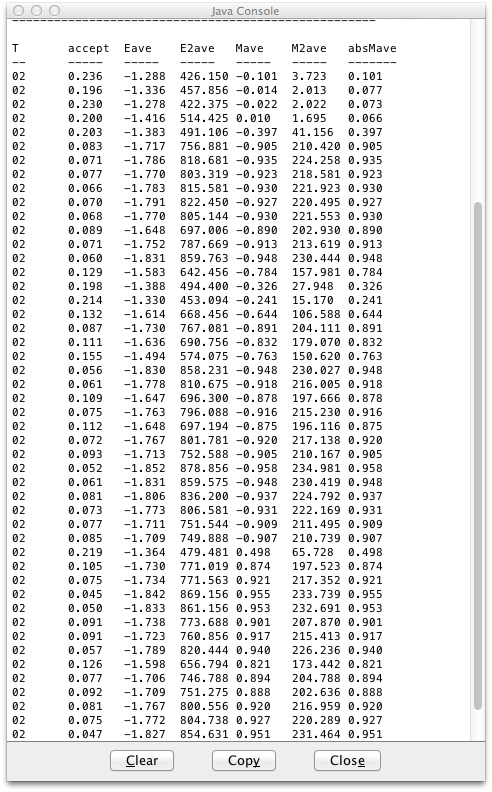
\includegraphics[width=.48\textwidth]{console.png}
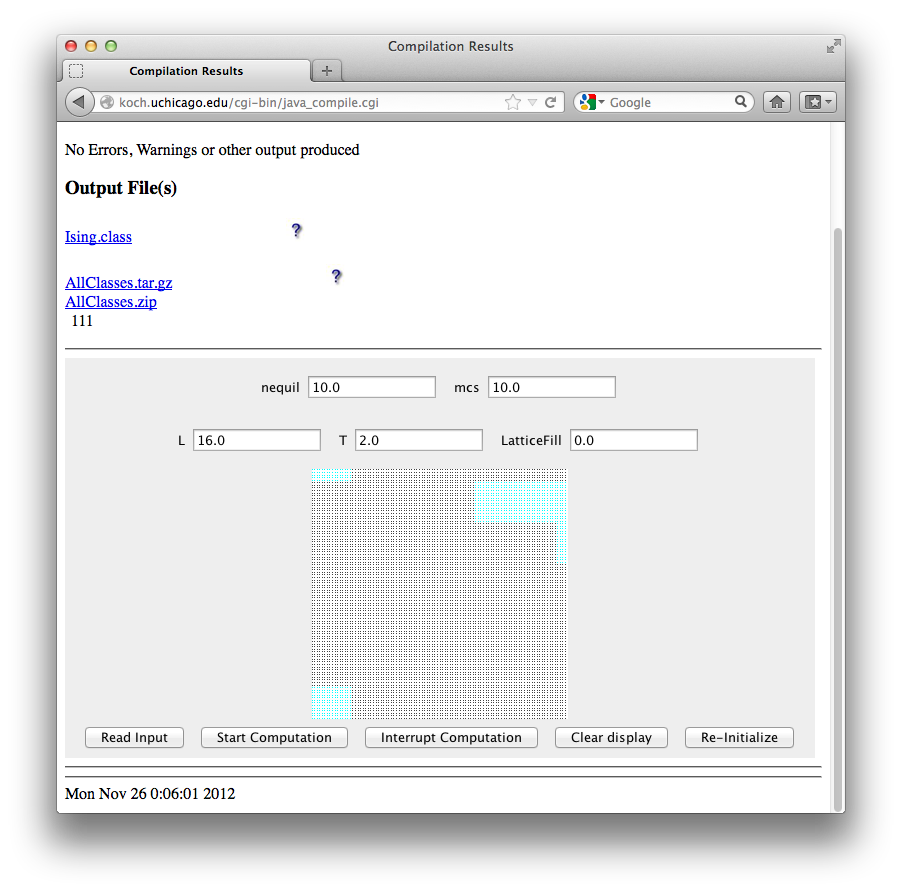
\includegraphics[width=.48\textwidth]{applet.png}
\end{figure}

So far, I have managed to port the BASIC code from Gould\&Tobochnik into java source code which runs and visualizes the Ising model using the Metropolis algorithm. The code is completely contained in \ttt{Ising.java}.

At the moment, system parameters such as temperature, initial spin config, and system size can be set by the user along with simulation parameters regarding the number of monte carlo steps per data point.

My code can calculate and output system properties such as energy and magnetization. Additionally, it can display the system on a 256x256 pixel grid (as long as L = $2^n <= 256$). There seems to be one slight trouble with this visualization (at the high end of either coordinate, there is only half a cell). However, this should be easily remedied with a review of my source code.

The next step is to implement the user-chosen measurement capabilities for central boxes in the system, as well as more thorough verification of the accuracy of my code.

\end{document} 
